\documentclass[oneside, abstracton, titlepage]{scrartcl}

\usepackage[left=2.5cm,right=2.6cm,top=3cm,bottom=3cm]{geometry}
\usepackage[utf8]{inputenc}
\usepackage[intlimits]{amsmath}
\usepackage{amssymb}
\usepackage{color}

\usepackage{graphicx}

\begin{document}
	\title{Discover governing reactions from concentration data}
	\maketitle
	
	\section*{Introduction}
	When presented with a time series of possibly noisy concentrations as output of, e.g.,  measurements or simulations that were parameterized by microscopic rates \textcolor{red}{(cite ReaDDy?)}, one can ask for the corresponding macroscopic rates and generating reaction network. 
	In this paper we present an application of the shallow learning method SINDy \cite{Brunton2015} which is able to identify generating parsimonious nonlinear dynamics in data that stems from dynamical systems.
	In our application we, opposed to the original method, do not only look for macroscopic rates of net species change but investigate the specific reactions that might have lead to the observations.
	We demonstrate the algorithm on a toy problem demonstrating the identification abilities.
	
	\section*{The method}
	The underlying model that we want to fit the data to is a law of mass action type dynamical system. To this end, let $S$ be the number of species, then the concentration data at a time $t$ can be represented by a vector
	\[
	\mathbf{x}(t)=\begin{pmatrix}
	x_1(t)\\ \vdots \\ x_S(t)
	\end{pmatrix}\in \mathbb{R}^S.
	\]
	Further, one can choose $R$ possible ansatz reactions with their respective reaction function
	\[
	\textbf{y}_r(\textbf{x}(t))=\begin{pmatrix}
	y_{r,1}(\textbf{x}(t)) \\ \vdots \\ y_{r,S}(\textbf{x}(t))
	\end{pmatrix}
	\]
	so that the change of concentration for species $i$ at time $t_i$, is represented by the dynamical system
	\[
	\dot{\textbf{x}}_i(t) = \sum_{r=1}^{R}y_{r,i}(\textbf{x}(t))\xi_r,\quad i=1,\ldots, S,
	\]
	where $\xi_r$ are the to-be estimated macroscopic rates.
	
	When presented with a time series with $T$ observations, the data can be represented as a matrix
	\[
	\textbf{X} = \begin{pmatrix}
		x_1(t_1) & x_2(t_1) & \cdots & x_S(t_1) \\
		x_1(t_2) & x_2(t_2) & \cdots & x_S(t_2) \\
		\vdots   & \vdots   & \ddots & \vdots   \\
		x_1(t_T) & x_2(t_T) & \cdots & x_S(t_T)
	\end{pmatrix} \in \mathbb{R}^{T\times S}.
	\]
	Given this matrix, one can propose a library $\Theta(\textbf{X}) = \begin{pmatrix} \theta_1(\textbf{X}) & \theta_2(\textbf{X}) & \cdots & \theta_R(\textbf{X}) \end{pmatrix}$ of $R$ ansatz reactions with corresponding reaction functions
	\[
	\theta_r(\textbf{X}) = \begin{pmatrix}
	\textbf{y}_r(\textbf{X}_1)^T \\ \vdots \\ \textbf{y}_r(\textbf{X}_T)^T
	\end{pmatrix}\in \mathbb{R}^{T\times S},\quad r=1,\ldots,R,
	\]
	where $\textbf{X}_i$ denotes the $i$-th row in $X$. Applying the concentration trajectory to the library yields a data tensor $\Theta(\textbf{X})\in\mathbb{R}^{T\times S\times R}$. Following the approach of SINDy, the goal is now to find coefficients $\Xi = \begin{pmatrix} \xi_1 & \xi_2 & \cdots & \xi_R
	\end{pmatrix}^T$, so that
	\[
	\dot{\textbf{X}} = \Theta(\textbf{X})\Xi = \sum_{r=1}^{R}\theta_r(\textbf{X})\xi_r.
	\]
	In particular, the system is linear in the coefficients $\Xi$, which makes sparse regression tools such as LASSO \cite{Tibshirani1996, Hastie2009} applicable. To this end, one can consider the minimization problem to find $\hat{\Xi}$ such that
	\begin{align}
		\hat{\Xi} = \underset{\Xi}{\arg\min}\left( \frac{1}{2T}\left\| \dot{\textbf{X}} - \Theta(\textbf{X})\Xi \right\|_F^2 + \alpha\|\Xi\|_1 \right) \quad \text{subject to }\Xi \geq 0,
	\label{method:minimizationproblem}\end{align}
	where $\alpha\geq 0$ is a sparsity inducing hyperparameter. For $\alpha=0$ this problem reduces to constrained least-squares. For solving (\ref{method:minimizationproblem}) we apply the sequential least squares minimizer SLSQP, originally described in \cite{Kraft1988}, contained in, e.g., the software package SciPy \cite{SciPy}.
	
	\section*{Examples}
	
	\begin{figure}
		\begin{center}
			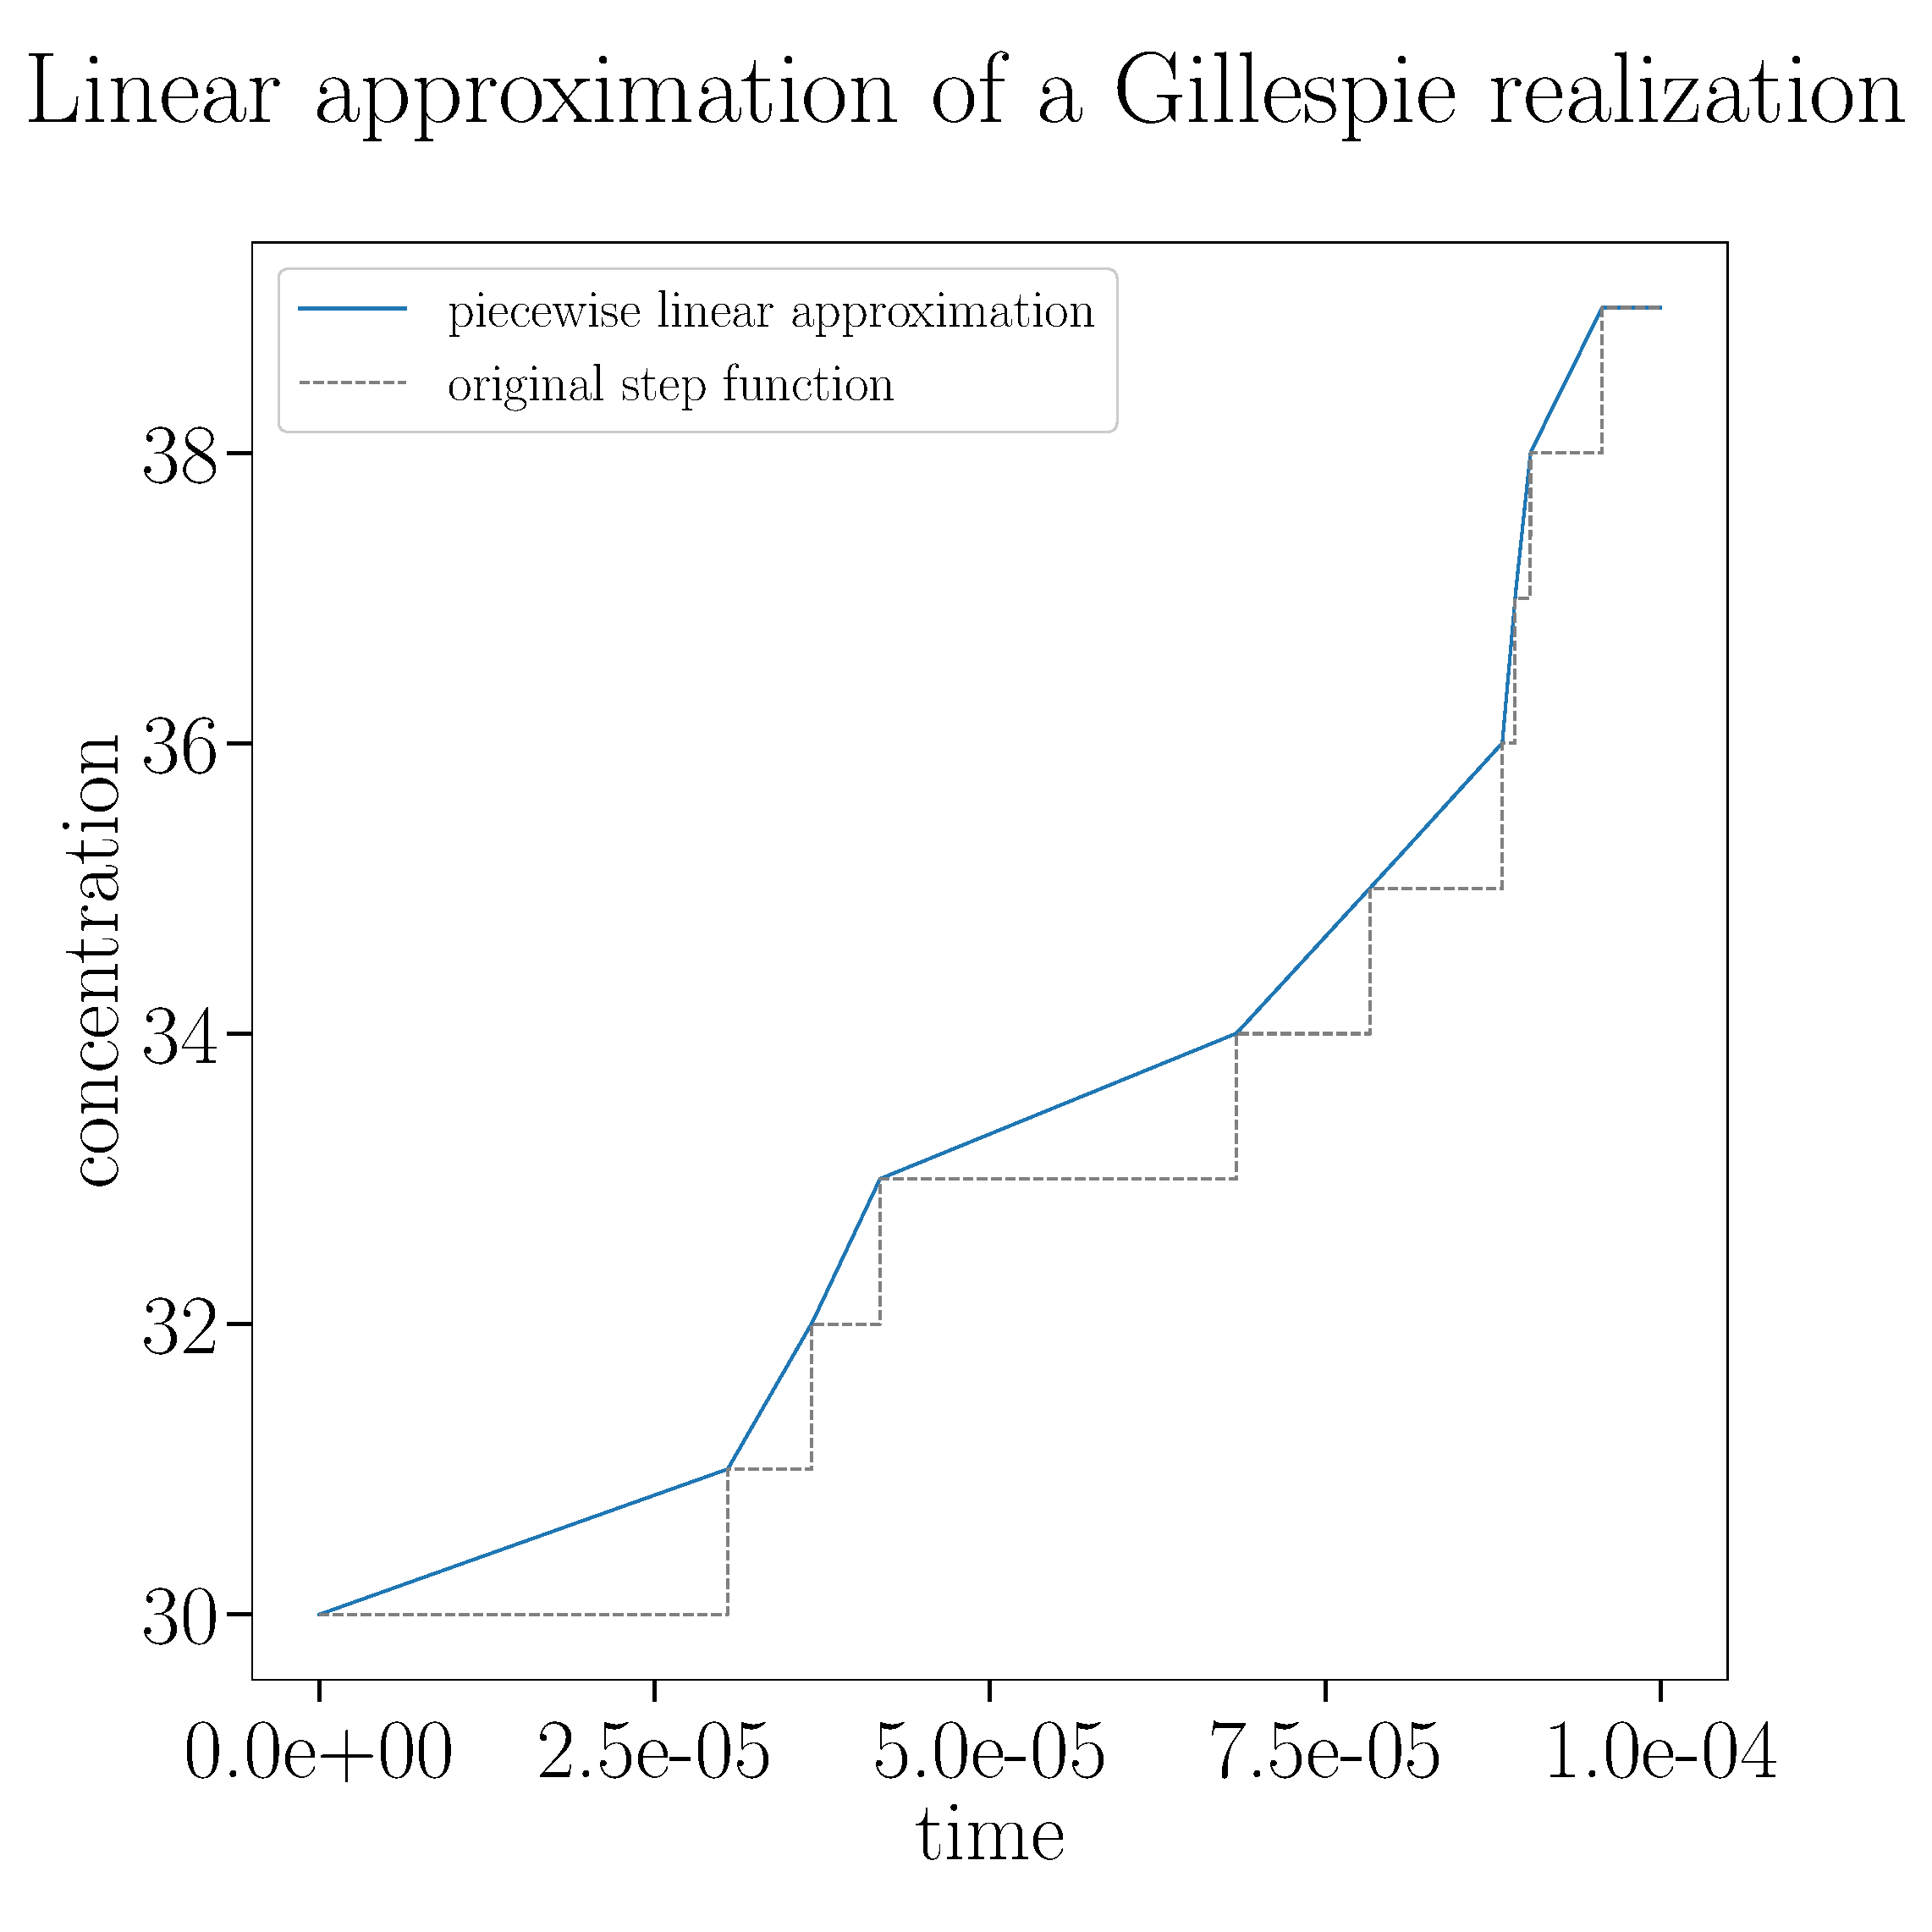
\includegraphics[width=.5\textwidth]{./figures_tex/aux_linear_approximation.eps}
		\end{center}
		\caption{This figure depicts a possible output yielded by an application of the Gillespie method and the performed piecewise linear approximation in order to obtain a better behaving derivative.}
		\label{examples:linear-approximation}
	\end{figure}
	
	For generating time series data of concentrations we use the Gillespie method \cite{Gillespie1976}. For a given set of initial conditions, we produce several realizations which are then converted to a trajectory with fixed time step and averaged. Since these trajectories are piecewise constant, one has to take special care when approximating the temporal derivative. Simply taking finite differences has the effect that, with decreasing time step, the derivative is most of the time constant zero and approaches infinity at the jump discontinuities. To counter this effect, we first perform a linear approximation between each two adjacent discontinuities, as depicted in Figure \ref{examples:linear-approximation}. (\textcolor{red}{Use regularized derivative?})
	
	\subsection*{Regression without regularization}
	
	
	\subsection*{Regression with regularization}
	
	\section*{Conclusion}
	dfdf
	
	
	\newpage
% 	\bibliographystyle{alpha}
	\bibliographystyle{abbrv}
	\bibliography{bibliography.bib}
	
\end{document}
